\documentclass[xcolor={usenames,dvipsnames,svgnames}, compress]{beamer}

\usepackage{booktabs}
\usepackage{dcolumn}
\usepackage{colortbl}
\usepackage{xcolor}
\usepackage{hyperref}
\usepackage{amsmath}
\usepackage{wrapfig}
\usepackage[style=authoryear-comp, backref=true]{biblatex}

%
% custom colors
\definecolor{untractable_red}{RGB}{209, 25, 25}
\definecolor{tractable_green}{RGB}{0, 153, 51}


\usetheme{enziteto}

\setbeamertemplate{headline}{}

\addbibresource{../referomnia/referomnia.bib}

\begin{document}

\newlength{\custombulletheight}
\setlength{\custombulletheight}{\dimexpr0.5\ht1-0.5\ht2}

\newcommand{\plusbullet}{\raisebox{\custombulletheight}{\hbox{\tiny\textcolor{lacamlilac}{$\boldsymbol{\oplus}$}}\hspace{-2pt}}}

\setbeamertemplate{itemize item}{\raisebox{.21ex}{\hbox{\tiny\textcolor{lacamlilac}{$\boldsymbol{\oplus}$}}\hspace{-2pt}}}
\setbeamertemplate{itemize subitem}{\raise .2ex\hbox{\tiny\textcolor{lacamlilac}{$\boldsymbol{\otimes}$}}\hspace{-3pt}}
\setbeamertemplate{itemize subsubitem}{\textcolor{lacamlilac}{$\oplus$}}
\setbeamertemplate{bibliography item}{\hspace{10pt}\raise .2ex\hbox{\tiny\textcolor{lacamlilac}{$\boldsymbol{\oplus}$}}}


% 
% custom bullets

% \renewcommand\labelitemi{\raisebox{\custombulletheight}{\hbox{\tiny\textcolor{lacamlilac}{$\boldsymbol{\oplus}$}}\hspace{-2pt}}}
\title{Simplifying, Regularizing and Strengthening Sum-Product Network Structure Learning}
\author{Antonio  Vergari, Nicola  {Di Mauro} and Floriana Esposito}
\institute{Lacam$@$DIB$@$Uniba}
\institute{Università degli Studi di Bari}
\department{Dipartimento di Informatica}
\laboratory{LACAM}
\group{Machine Learning}
\institutelogo{
\includegraphics[width=25pt]{figures/unibaba}}
\lablogo{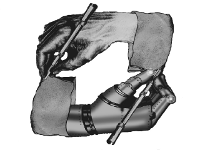
\includegraphics[width=35pt]{figures/lacam}}


{
  \setbeamertemplate{headline}{}
  \setbeamertemplate{footline}{}
  \begin{frame}
    \titlepage
  \end{frame}
}

\begin{frame}
  \frametitle{Summary}
  \begin{itemize}
  \item Sum-Product Networks refresher
  \item Why and How Structure learning
  \item Simplifying by limiting splits
  \item Regulizing by effective early stopping
  \item Strengthening by model averaging
    \item Conclusions and further works
  \end{itemize}
\end{frame}


\begin{frame}[t]
  \frametitle{PGMs and Tractability}
  \begin{table}[!ht]
    \setlength{\tabcolsep}{25pt}
    \centering
    \begin{tabular}{c c}
      
      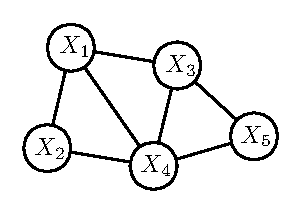
\includegraphics[width=0.33\linewidth]{figures/mrf} &
                                                            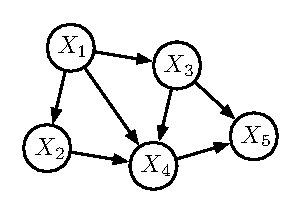
\includegraphics[width=0.33\linewidth]{figures/bn}\\
      \addlinespace[-0.2cm]
      \scriptsize  $P(\mathbf{X})=\frac{1}{Z}\prod_{c}\phi_{c}(\mathbf{X}_{c})$
                                                          & 
      \scriptsize
                                                            $P(\mathbf{X})=\prod_{i=1}^nP(X_{i}|\mathbf{Pa}_{i})$\\
      \addlinespace[0.5cm]
      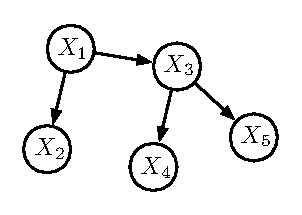
\includegraphics[width=0.33\linewidth]{figures/clt} &
                                                            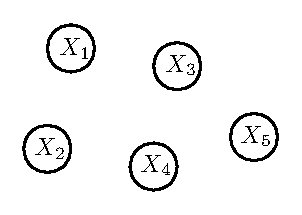
\includegraphics[width=0.33\linewidth]{figures/nf}\\
      \addlinespace[-0.2cm]
      \scriptsize
      $P(\mathbf{X})=\prod_{i=1}^nP(X_{i}|Pa_{i})$ &
      \scriptsize $P(\mathbf{X})=\prod_{i=1}^nP(X_{i})$                                                              
    \end{tabular}
  \end{table}
  %\footnotesize Inference on Probabilistic Graphical Models (PGMs) is generally untractable.
\end{frame}

\begin{frame}[t]
  \frametitle{PGMs and Tractability}
  \begin{table}[!ht]
    \setlength{\tabcolsep}{25pt}
    \centering
    \begin{tabular}{c c}
      
      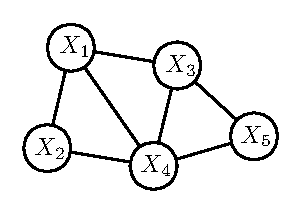
\includegraphics[width=0.33\linewidth]{figures/mrf} &
                                                            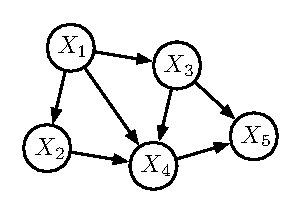
\includegraphics[width=0.33\linewidth]{figures/bn}\\
      \addlinespace[-0.2cm]
      \scriptsize\color{untractable_red}  \textbf{\emph{untractable}} & \scriptsize\color{untractable_red} \textbf{\emph{untractable}} \\
      \addlinespace[0.5cm]
      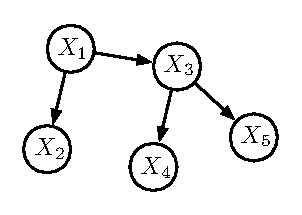
\includegraphics[width=0.33\linewidth]{figures/clt} &
                                                            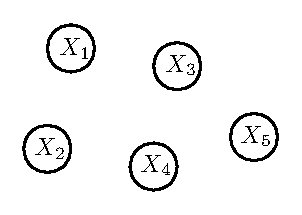
\includegraphics[width=0.33\linewidth]{figures/nf}\\
      \addlinespace[-0.2cm]
      \scriptsize\color{tractable_green} \emph{\textbf{tractable}} & \scriptsize\color{tractable_green} \emph{\textbf{tractable}}                                                              
    \end{tabular}
  \end{table}
  %\footnotesize To guarantee polynomial inference, tractable models trade off model expressiveness.
\end{frame}

\begin{frame}[t]
  \frametitle{Sum-Product Networks (I)}
  \footnotesize
   SPNs are DAGs \emph{compiling} the partition function of a joint pdf into a \textbf{\emph{deep}} architecture of \textbf{sum}
   and \textbf{product} nodes.\par\bigskip

   Product nodes define factorizations over independent components, sum
   nodes weighted mixtures. Leaves are tractable univariate distributions.\par\bigskip

   \begin{minipage}{0.45\linewidth}
    \centering
    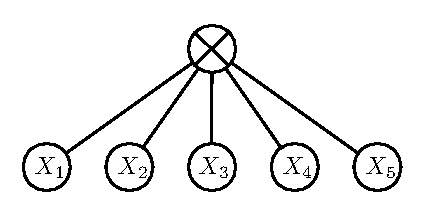
\includegraphics[width=0.72\linewidth]{figures/spn-prod}\\
    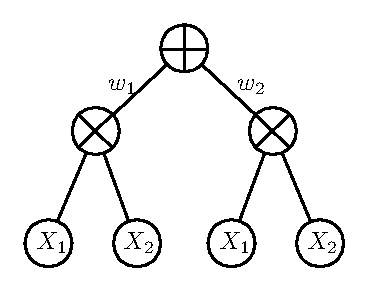
\includegraphics[width=0.653\linewidth]{figures/spn-sum}
  \end{minipage}%
  \begin{minipage}{0.5\linewidth}
    \vspace{7pt}
    % \footnotesize
    % SPNs are DAGs \emph{compiling} the partition function of a joint pdf into a \textbf{\emph{deep}} architecture of \textbf{sum}
    % and \textbf{product} nodes.\\

    % Product nodes define factorizations over independent components, sum
    % nodes mixtures. Leaves are tractable univariate distributions.\\

    %Sum node children weights are the parameters of the model.\\

    Products over nodes with different scopes (\emph{decomposability}) and
    sums over nodes with same scopes (\emph{completeness}) guarantee modeling
    a pdf (\emph{validity}).\par\bigskip

    The size of the network is the number of edges in it.\par\bigskip

    The depth of the network is the number of alternated layers.\par\bigskip

    % Considering only valid SPNs of \emph{alternated layers of sum and products}.

    

    

  \end{minipage}
\end{frame}

\begin{frame}
  \frametitle{Sum-Product Networks (II)}
  \begin{minipage}{0.45\linewidth}
    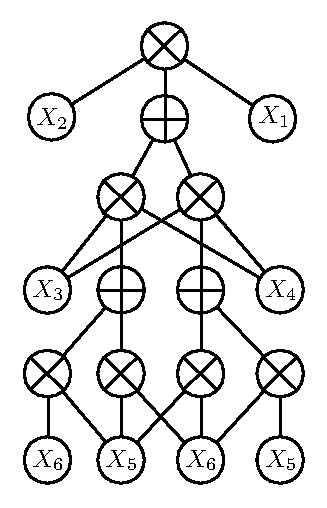
\includegraphics[width=0.8\linewidth]{figures/spn-long}
  \end{minipage}\begin{minipage}{0.55\linewidth}
    \footnotesize
    Bottom-up evaluation of the network: \\

    $S_{X_i}(x_j)=P(X_i=x_j)$
    
    $S_{+}(\mathbf{x})=\sum\limits_{i\in ch(+)}w_{i}S_{i}(\mathbf{x})$

    $S_{\times}(\mathbf{x})=\prod\limits_{i\in
      ch(\times)}S_{i}(\mathbf{x})$
    
    Inferences linear in the size of the network (\# edges):
    \begin{itemize}
    \item $Z = S(*)$
    \item $P(\mathbf{e}) = S(\mathbf{e})/S(*)$
    \item $P(\mathbf{q}| \mathbf{e}) = \frac{P(\mathbf{q},
        \mathbf{e})}{P(\mathbf{e})} = \frac{S(\mathbf{q},
        \mathbf{e})}{S(\mathbf{e})}$
    \item $MPE(\mathbf{q},\mathbf{e}) = \max_{\mathbf{q}}P(\mathbf{q}, \mathbf{e}) = S^{max}(\mathbf{e})$  
    \end{itemize}
     
    
    
  \end{minipage}
\end{frame}

\begin{frame}
  \frametitle{How and Why Structure Learning}
  \footnotesize
  Fixed structures are hard to engineer and train (fully connected layers).\par\bigskip
  
  Automatic discovery of latent vars.\par\bigskip

   Constraint-based search formulation. Discover hidden variables for sum node mixtures and independences
  for product node components:
  \begin{itemize}
    \itemsep 6pt
  \item greedy top-down: KMeans on features~\emph{\parencite{Dennis2012}}; alternating clustering on
    instances and independence tests on features, \textbf{LearnSPN}~\emph{\parencite{Gens2013}}

  \item greedy bottom up: merging feature regions by a \emph{Bayesian-Dirichlet independence test},  and reducing edges by maximizing MI\emph{~\parencite{Peharz2013}}

  

  \item \textbf{ID-SPN}: turning LearnSPN in log-likelihood guided expansion of sub-networks
    approximated by Arithmetic Circuits~\emph{\parencite{Rooshenas2014}}

  \end{itemize}
  \vspace{6pt}

  
\end{frame}

\begin{frame}
  \frametitle{Why Structure Quality Matters}

  \footnotesize
  
  Tractability is guaranteed if the network size is polynomial in \#
  vars.\par\bigskip

  Comparing network sizes is better than comparing inference times.\par\bigskip

  Deeper networks are possibly more expressively efficient~\parencite{Martens2014,Zhao2015}\par\bigskip

  Overcomplex networks do not  generalize well\par\bigskip
  
  Structure quality desiderata: smaller but accurate, deeper but not
  wider, SPNs

  
  
\end{frame}

\begin{frame}
  \frametitle{LearnSPN (I)}
  \footnotesize
  Build a tree-like SPN by recursively split the data matrix:

  \begin{itemize}
  \item splitting columns into pairs by a greedy \textbf{\emph{G Test}} based
    procedure with threshold $\rho$:
    \[
    G(X_i, X_j) =  2\sum_{x_i \sim X_i}\sum_{x_j \sim X_j}c(x_i, x_j)\cdot \log\frac{c(x_i, x_j)\cdot |T|}{c(x_i)c(x_j)}
    \]
  \item clustering instances with \textbf{\emph{online Hard-EM}} with cluster penalty
    $\lambda$:
    \[\begin{array}{cc}
        Pr(\mathbf{X})= \sum_{C_i \in \mathbf{C}}\prod_{X_j \in \mathbf{X}}Pr(X_j|C_i)Pr(C_i)\\
        % & Pr(C_i) \propto e^{-\lambda |\mathbf{C}|\cdot |\mathbf{X}|}\\
      \end{array}\]
  \item if there are less than $m$ instances, put a \textbf{\emph{naive
    factorization}} over leaves
  \item each univariate distribution get \emph{\textbf{ML estimation}} smoothed by $\alpha$  
  \end{itemize}
  
  % \textbf{Online Hard-EM} with restarts to cluster instances $T$ with an exp prior ($Pr(C_i) \propto e^{-\lambda |\mathbf{C_i}|\cdot |\mathbf{X}|}$) on clusters to avoid overfitting:
  % \[\begin{array}{cc}
  %     Pr(\mathbf{X})= \sum_{C_i \in \mathbf{C}}\prod_{X_j \in \mathbf{X}}Pr(X_j|C_i)Pr(C_i)\\
  %     % & Pr(C_i) \propto e^{-\lambda |\mathbf{C}|\cdot |\mathbf{X}|}\\
  %   \end{array}\]
  %   found clusters become \emph{sum node children} with parameters $w_i = |C_i|/|T|$.\par
  %   \vspace{\baselineskip}
  %   Features $\mathbf{X}$ are clustered into independent components via a greedy procedure based on a \textbf{G Test} over pairs $X_i$,$X_j$:
  %   \[
  %   G(X_i, X_j) =  2\sum_{x_i \sim X_i}\sum_{x_j \sim X_j}c(x_i, x_j)\cdot \log\frac{c(x_i, x_j)\cdot |T|}{c(x_i)c(x_j)}
  %   \]
  %   which are associated to \emph{product node children}.\par %\par
  %   % \vspace{\baselineskip}
  %   If $|T|<m$ consider features independent and create \emph{leaves} by \textbf{smooth laplacian frequence estimation} (with parameter $\alpha$).

\end{frame}

\begin{frame}
  % \frametitle{LearnSPN (II)}
  \begin{table}[ht]
    \centering
    \begin{tabular}{l l l l}
      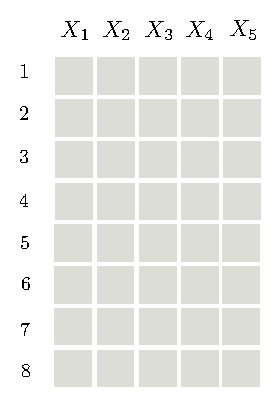
\includegraphics[width=0.228\linewidth]{figures/grid-0}&
                                                              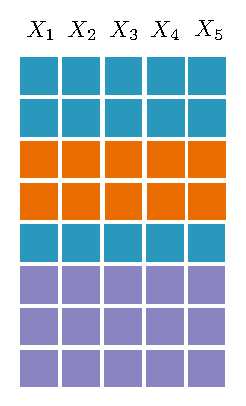
\includegraphics[width=0.2\linewidth]{figures/grid-1}&
                                                                                                                      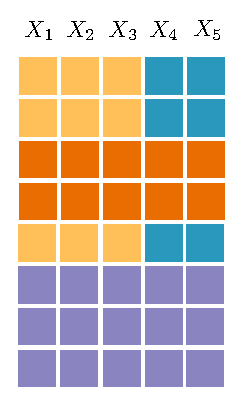
\includegraphics[width=0.2\linewidth]{figures/grid-2}&
                                                                                                                                                                              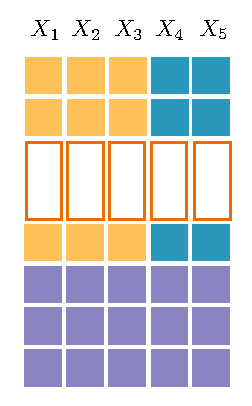
\includegraphics[width=0.208\linewidth]{figures/grid-3}\\
    \end{tabular}
  \end{table}
  \hfill\
  %{\raggedright
    \begin{table}[ht]
       \begin{tabular}{r r r}
         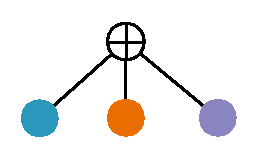
\includegraphics[width=0.2\linewidth]{figures/learnspn-1}&
                                                                     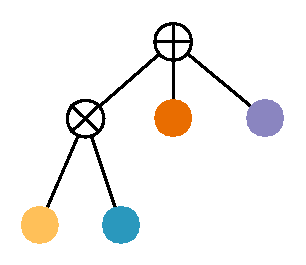
\includegraphics[width=0.24\linewidth]{figures/learnspn-2}&
                                                                                                                                 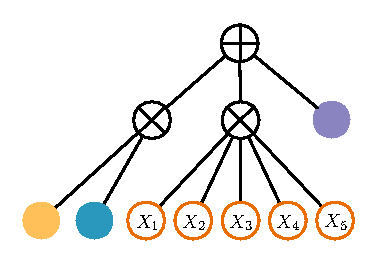
\includegraphics[width=0.30\linewidth]{figures/learnspn-3}\\
      \end{tabular}
    \end{table}
  %}
\end{frame}

\begin{frame}
  \frametitle{Symplifying by limiting node splits}
  \footnotesize
  \textsf{LearSPN} performs two interleaved \textbf{\emph{greedy
      hierarchical}} divisive \textbf{\emph{clustering}}
  processes (co-clustering).\par\bigskip

  Each process benefits from the other one improvements/highly suffers
  from other's mistakes.\par\bigskip

  Idea: slowing down the processes by limiting the number of
  nodes to split into. \textsf{SPN-B}, variant of \textsf{LearnSPN} that uses EM
  for mixture modeling with
  $k=2$ to cluster rows.\par\bigskip

  Pros:
  \begin{itemize}
  \item not committing to complex structures too early  
  \item same expressive power: successive splits allow for more node children
  \item reducing node out fan increases the depth
  \item same accuracy, smaller networks
  \end{itemize}
  
\end{frame}

\begin{frame}
  \frametitle{Experimental setting}
  \footnotesize
Classical setting for \emph{\textbf{generative}} graphical models
structure learning \parencite{Gens2013}:
  \begin{itemize}
    \itemsep 7pt
  \item comparing the \emph{\textbf{average log-likelihood}} on predicting instances from a test set
  \item 19 binary datasets from classification, recommendation,
    frequent pattern mining\dots \parencite{Lowd2010} \parencite{Haaren2012}
    \item Training 75\% Validation 10\% Test 15\%  splits (no cv)
  \item Model selection via \textit{grid search} in the same parameter space:
    \begin{itemize}
      \footnotesize
    \item $\lambda \in \{0.2, 0.4, 0.6, 0.8\}$,
    \item $\rho \in \{5, 10, 15, 20\}$, 
    \item $m \in \{1, 50, 100, 500\}$, 
    \item $\alpha \in \{ 0.1, 0.2, 0.5, 1.0, 2.0\}$
    \end{itemize}
  \item comparing our variants against \textsf{LearnSPN},
    \textsf{ID-SPN} and \textsf{MT}~\parencite{Meila2000}
  \end{itemize}

\end{frame}
\begin{frame}
  \frametitle{Depth VS Size}
  \begin{table}[ht]
    \centering
    \begin{tabular}{c c}
      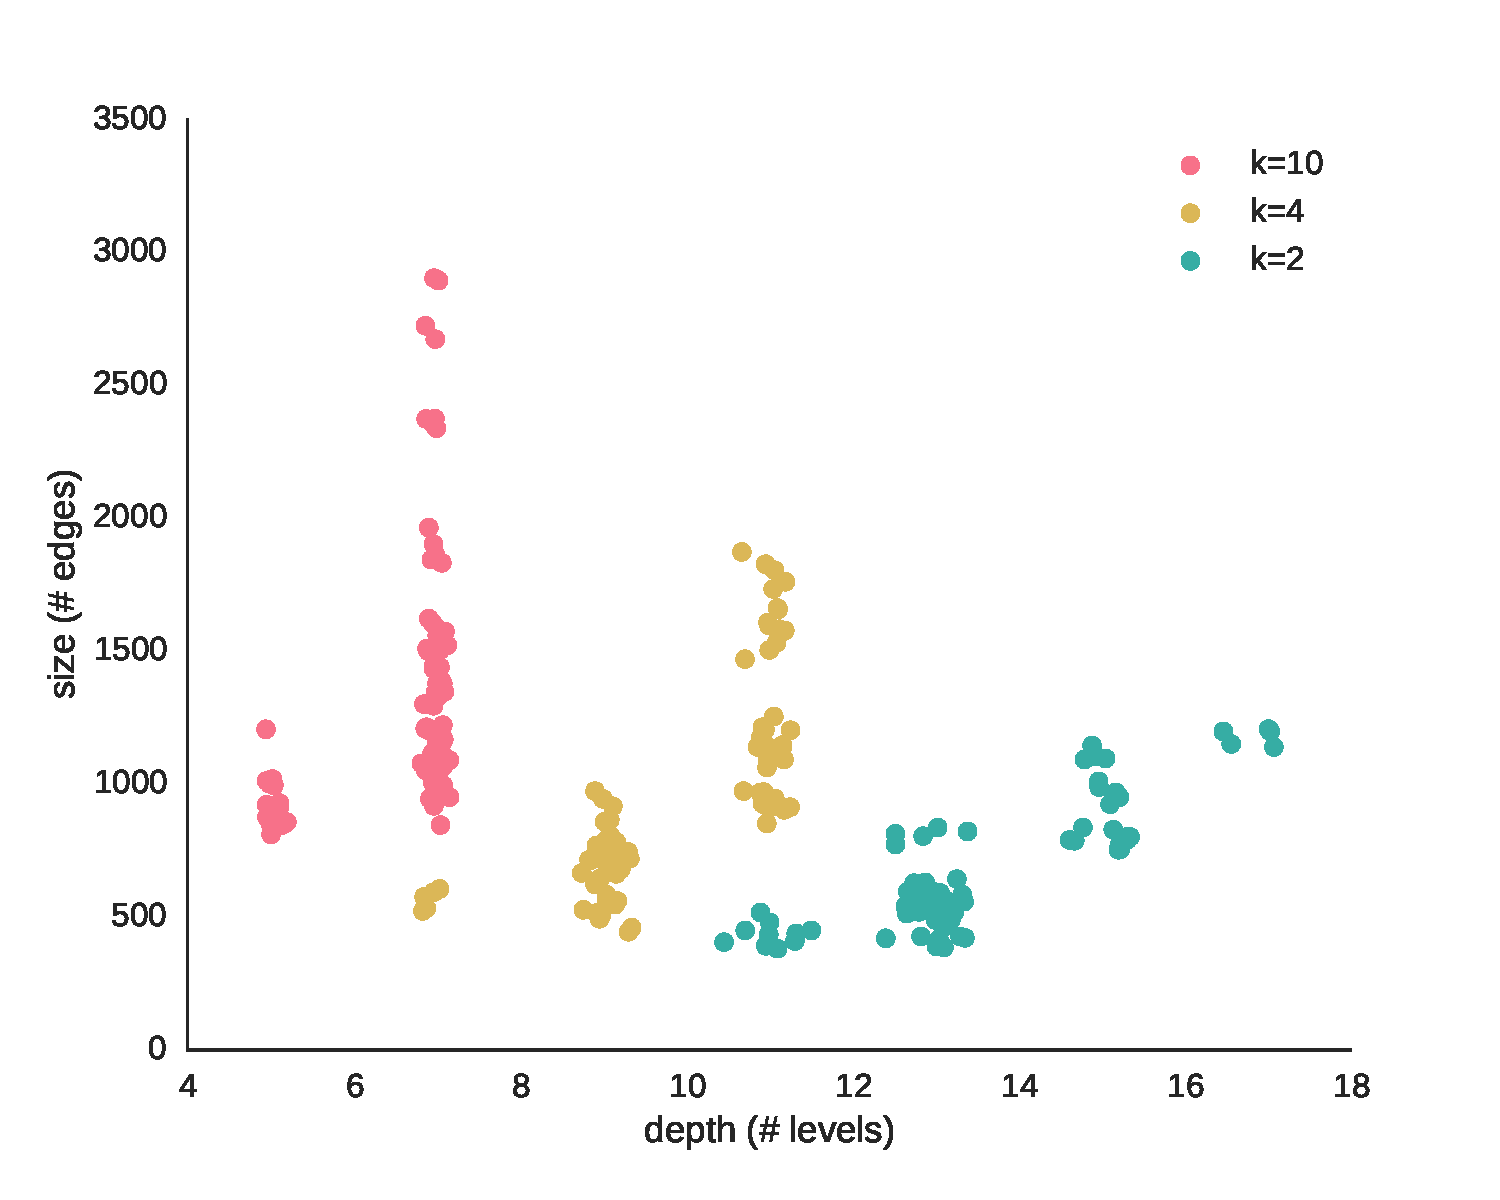
\includegraphics[width=0.45\linewidth]{figures/nltcs-depth.pdf}&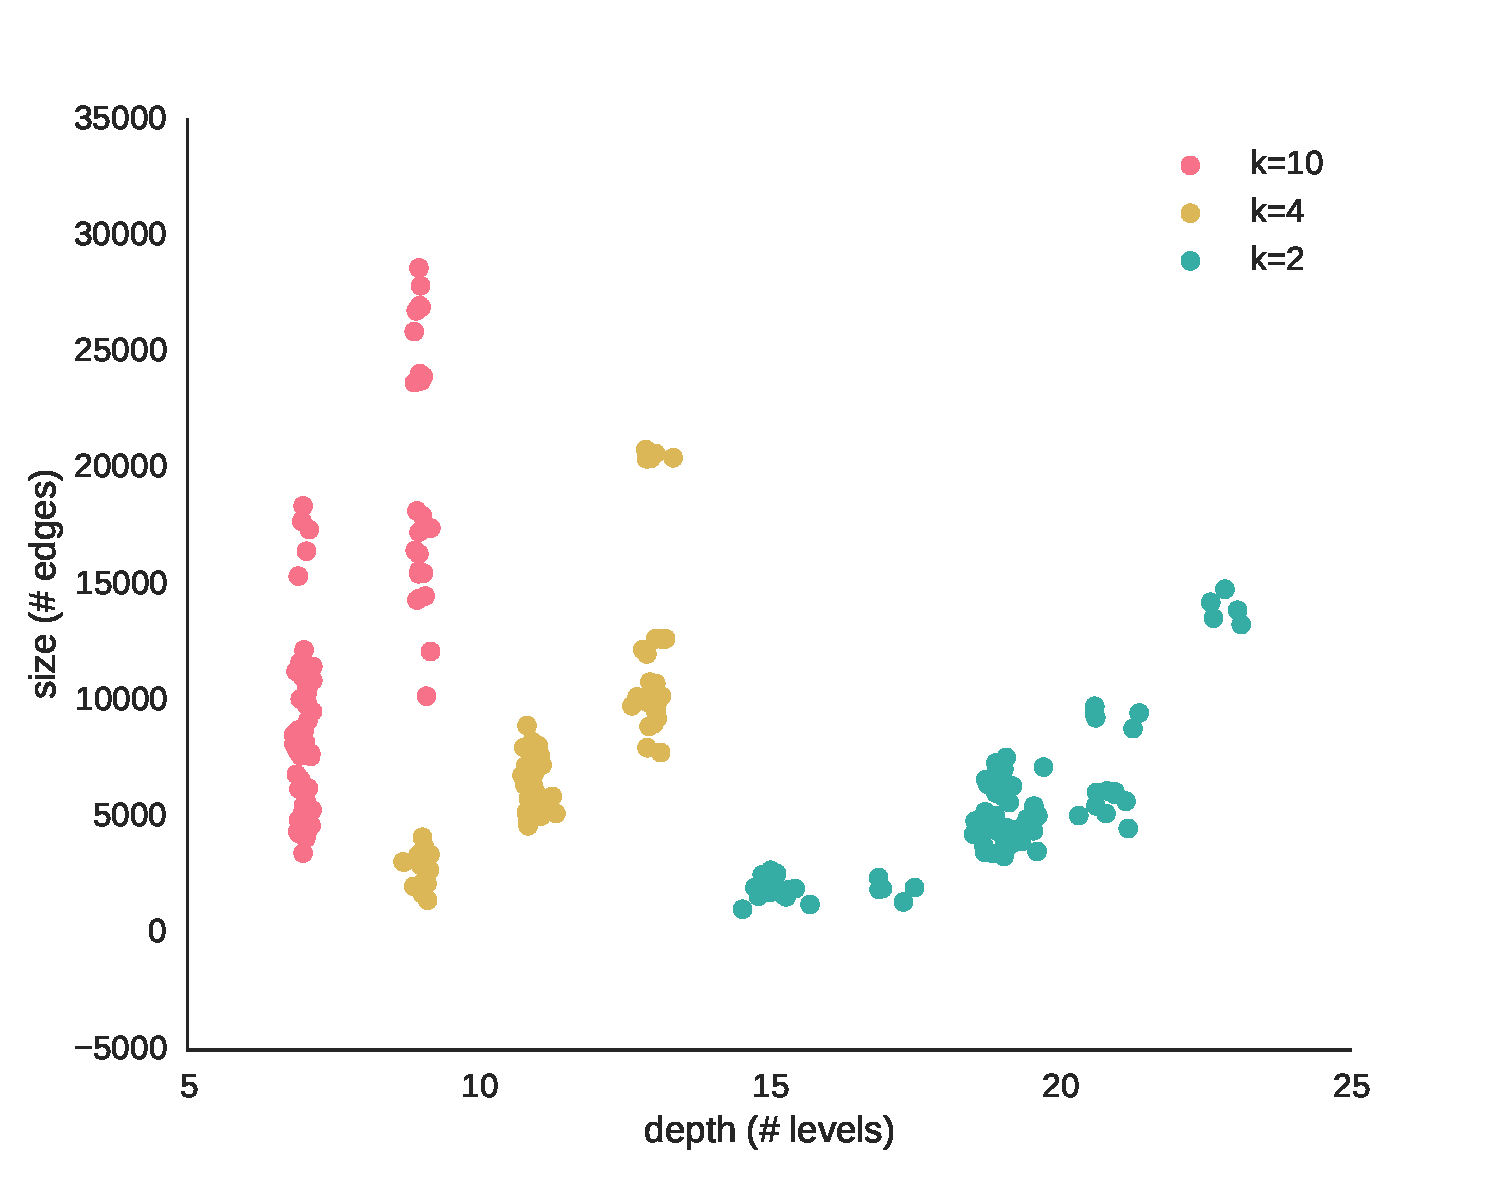
\includegraphics[width=0.45\linewidth]{figures/plants-depth.pdf}
    \end{tabular}
  \end{table}
\end{frame}

\begin{frame}
  \frametitle{Regularizing by effective early stopping}
  \footnotesize
  LearnSPN regularization is governed by $\alpha$ and $m$, however can
  be very ineffective:
  \begin{itemize}
  \item naive factorizations are too strong assumptions
    \item best likelihood structures prefer smaller values for $m$ to
      get accurate naive factorizations
    \end{itemize}\bigskip

    
    
    Substituting naive factorizations with Bayesian trees as leaf
    distributions $P(\mathbf{X}) = \prod_{j}P(X_j|Pa_{j})$:
    \begin{wrapfigure}{l}{0.35\textwidth}
      \vspace{-20pt}
      \begin{center}
        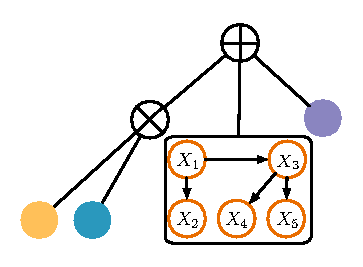
\includegraphics[width=0.35\textwidth]{figures/spn-clt}
      \end{center}
      \vspace{-20pt}
    \end{wrapfigure}
    \begin{itemize}
    \item learnable with Chow-Liu algorithm
    \item still tractable multivariate distributions for marginals,
      conditionals and MPE
    \item same or higher accuracy
    \item less complex structures for larger values of $m$
    \end{itemize}
\end{frame}

\begin{frame}
  \frametitle{Early stopping exp}
  \begin{table}[ht]
    \centering
    \begin{tabular}{c c}
      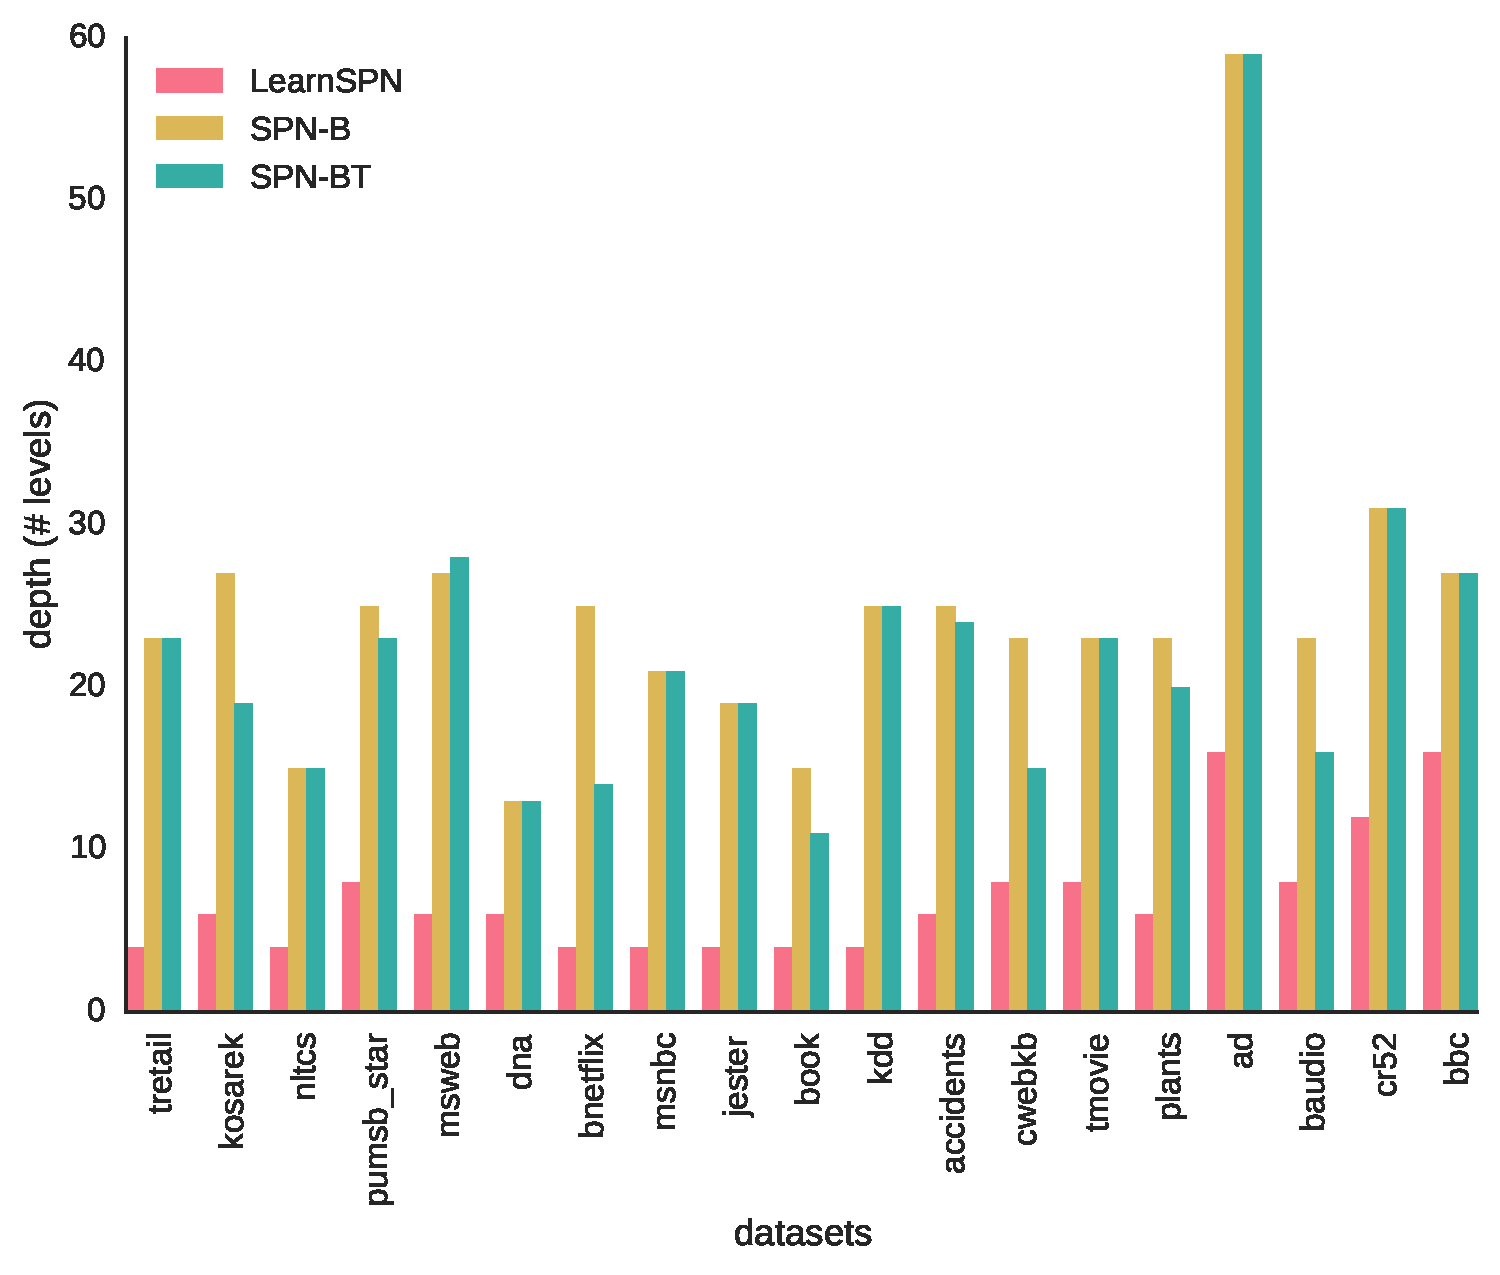
\includegraphics[width=0.45\linewidth]{figures/levels-comp}&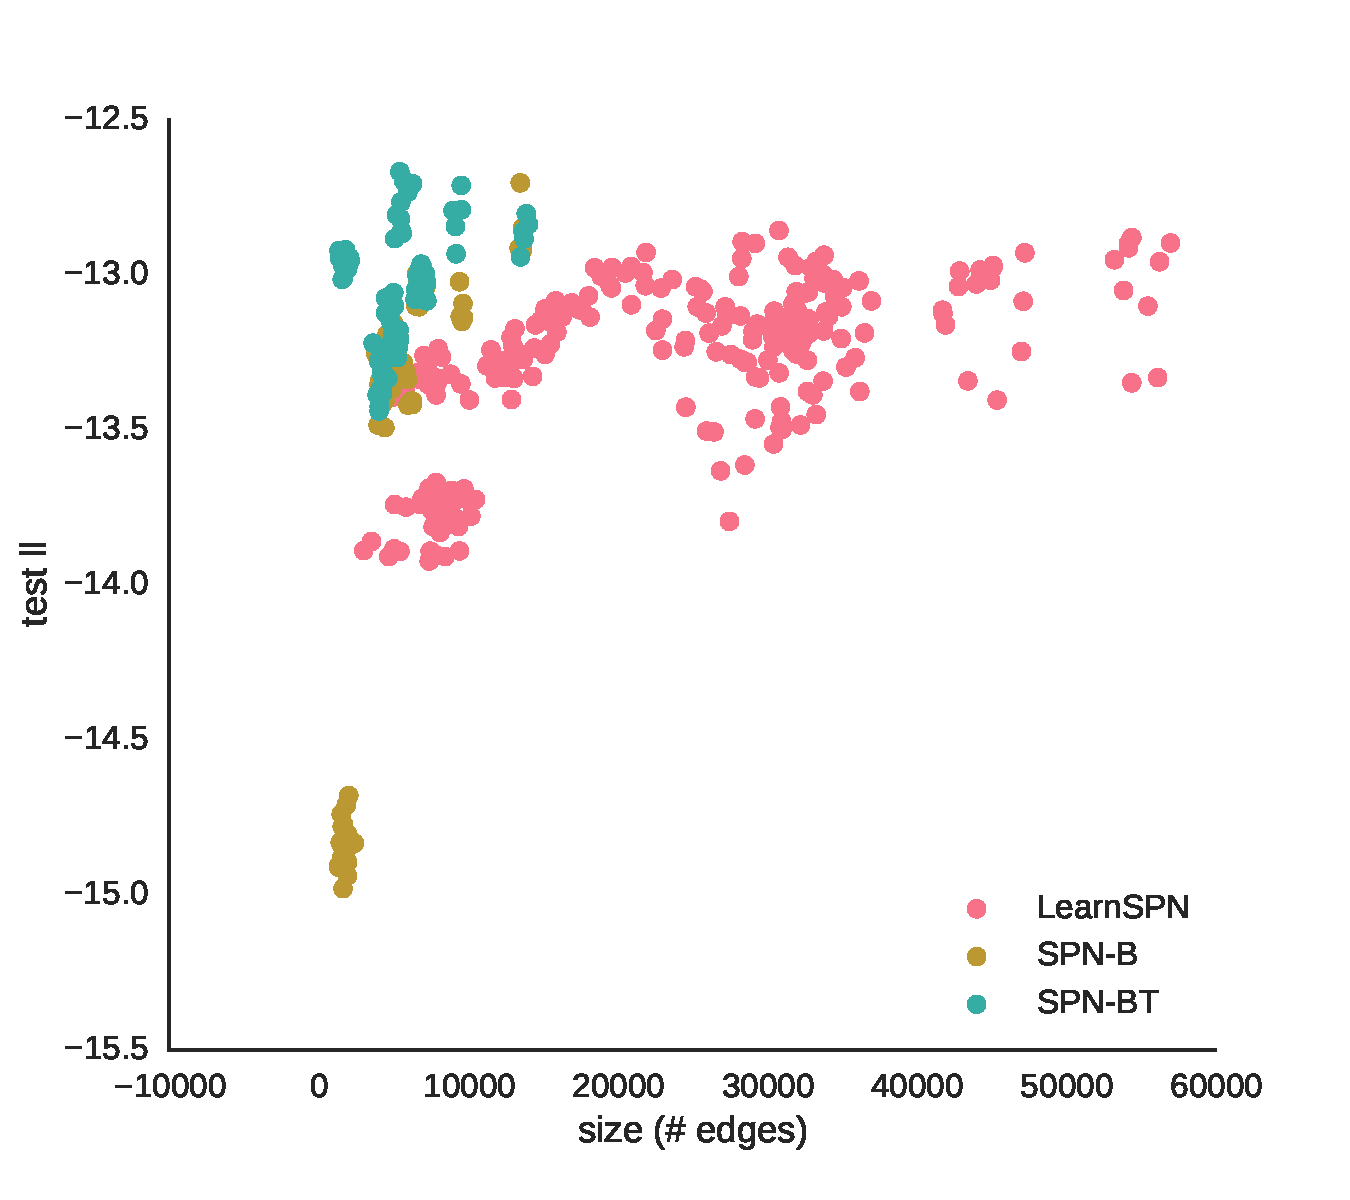
\includegraphics[width=0.45\linewidth]{figures/plants-ll-depth}
    \end{tabular}
  \end{table}

\end{frame}

\begin{frame}
  \frametitle{Strengthening by model averaging}
  \footnotesize
  Interpreting sum nodes as \emph{general additive estimators}. Leveraging
  classic statistical tools to learn them:
  \textbf{\emph{bagging}}.\par\bigskip

  Draw $k$ bootstrapped samples from the data, then grow an SPN $S_{B_i}$ on
  each of them. Join them into a single SPN $\hat{S}$ with a sum node:
  $$\hat{S}=\sum_{i=1}^{k}\frac{1}{k}S_{B_{i}}$$

  More robustness and less variance in the model.\par\bigskip

  Exponential number of nodes if done for each sum node (bootstrapping
  only at the root).\par\bigskip

  Two variants in the experiments: \textsf{SPN-BB} and
  \textsf{SPN-BTB}, whether Chow-Liu trees are employed or not.

  
\end{frame}

\begin{frame}
  \frametitle{LL exp}
  \tiny
  \begin{table}[!htbp]
    \centering
     \setlength{\tabcolsep}{3pt}  
    \begin{tabular}{r r r r r r r r}
      \toprule
      & \textsf{LearnSPN} & \textsf{SPN-B} & \textsf{SPN-BT} & \textsf{ID-SPN}  & \textsf{SPN-BB}   & \textsf{SPN-BTB}  & \textsf{MT}      \\
      \midrule                                                                                     
      \textbf{NLTCS}      & -6.110            & -6.048         & -6.048          & \textbf{-5.998}  & -6.014            & -6.014            & -6.008           \\
      \textbf{MSNBC}      & -6.099            & -6.040         & -6.039          & -6.040           & \textbf{-6.032}   & -6.033            & -6.076           \\
      \textbf{KDDCup2k}   & -2.185            & -2.141         & -2.141          & -2.134           & -2.122            & \textbf{-2.121}   & -2.135           \\
      \textbf{Plants}     & -12.878           & -12.813        & -12.683         & -12.537          & -12.167           & \textbf{-12.089}  & -12.926          \\
      \textbf{Audio}      & -40.360           & -40.571        & -40.484         & -39.794          & -39.685           & \textbf{-39.616}  & -40.142          \\
      \textbf{Jester}     & -53.300           & -53.537        & -53.546         & \textbf{-52.858} & \textbf{-52.873}  & -53.600           & -53.057          \\
      \textbf{Netflix}    & -57.191           & -57.730        & -57.450         & \textbf{-56.355} & -56.610           & \textbf{-56.371}  & -56.706          \\
      \textbf{Accidents}  & -30.490           & -29.342        & -29.265         & \textbf{-26.982} & -28.510           & -28.351           & -29.692          \\
      \textbf{Retail}     & -11.029           & -10.944        & 10.942          & \textbf{-10.846} & -10.858           & -10.858           & \textbf{-10.836} \\
      \textbf{Pumsb-star} & -24.743           & -23.315        & -23.077         & \textbf{-22.405} & -22.866           & -22.664           & -23.702          \\
      \textbf{DNA}        & -80.982           & -81.913        & -81.840         & -81.211          & -80.730           & \textbf{-80.068}  & -85.568          \\
      \textbf{Kosarek}    & -10.894           & -10.719        & -10.685         & -10.599          & -10.690           & \textbf{-10.578}  & -10.615          \\
      \textbf{MSWeb}      & -10.108           & -9.833         & -9.838          & -9.726           & -9.630            & \textbf{-9.614}   & -9.819           \\
      \textbf{Book}       & -34.969           & -34.306        & -34.280         & -34.136          & -34.366           & \textbf{-33.818}  & -34.694          \\
      \textbf{EachMovie}  & -52.615           & -51.368        & -51.388         & -51.512          & \textbf{-50.263}  & \textbf{-50.414}  & -54.513          \\
      \textbf{WebKB}      & -158.164          & -154.283       & -153.911        & -151.838         & -151.341          & \textbf{-149.851} & -157.001         \\
      \textbf{Reuters-52} & -85.414           & -83.349        & -83.361         & -83.346          & \textbf{-81.544}  & -81.587           & -86.531          \\
      % \textbf{20 NewsG}  & -155.218          & -152.846       & -153.072        & -151.467         &                   &                   & -154.367         \\
      \textbf{BBC}        & -249.466          & -247.301       & -247.254        & -248.929         & \textbf{-226.359} & \textbf{-226.560} & -259.962         \\
      \textbf{Ad}         & -19.760           & -16.234        & -15.885         & -19.053          & -13.785           & \textbf{-13.595}  & -16.012          \\
      \bottomrule
    \end{tabular}
    \caption[Experimentation results]{Average test
      log likelihoods for all algorithms.}
    \label{tab:resexp}
  \end{table}

\end{frame}
\begin{frame}
  \frametitle{Bagging exp}
  \begin{table}[ht]
    \centering
    \begin{tabular}[t]{c c}
      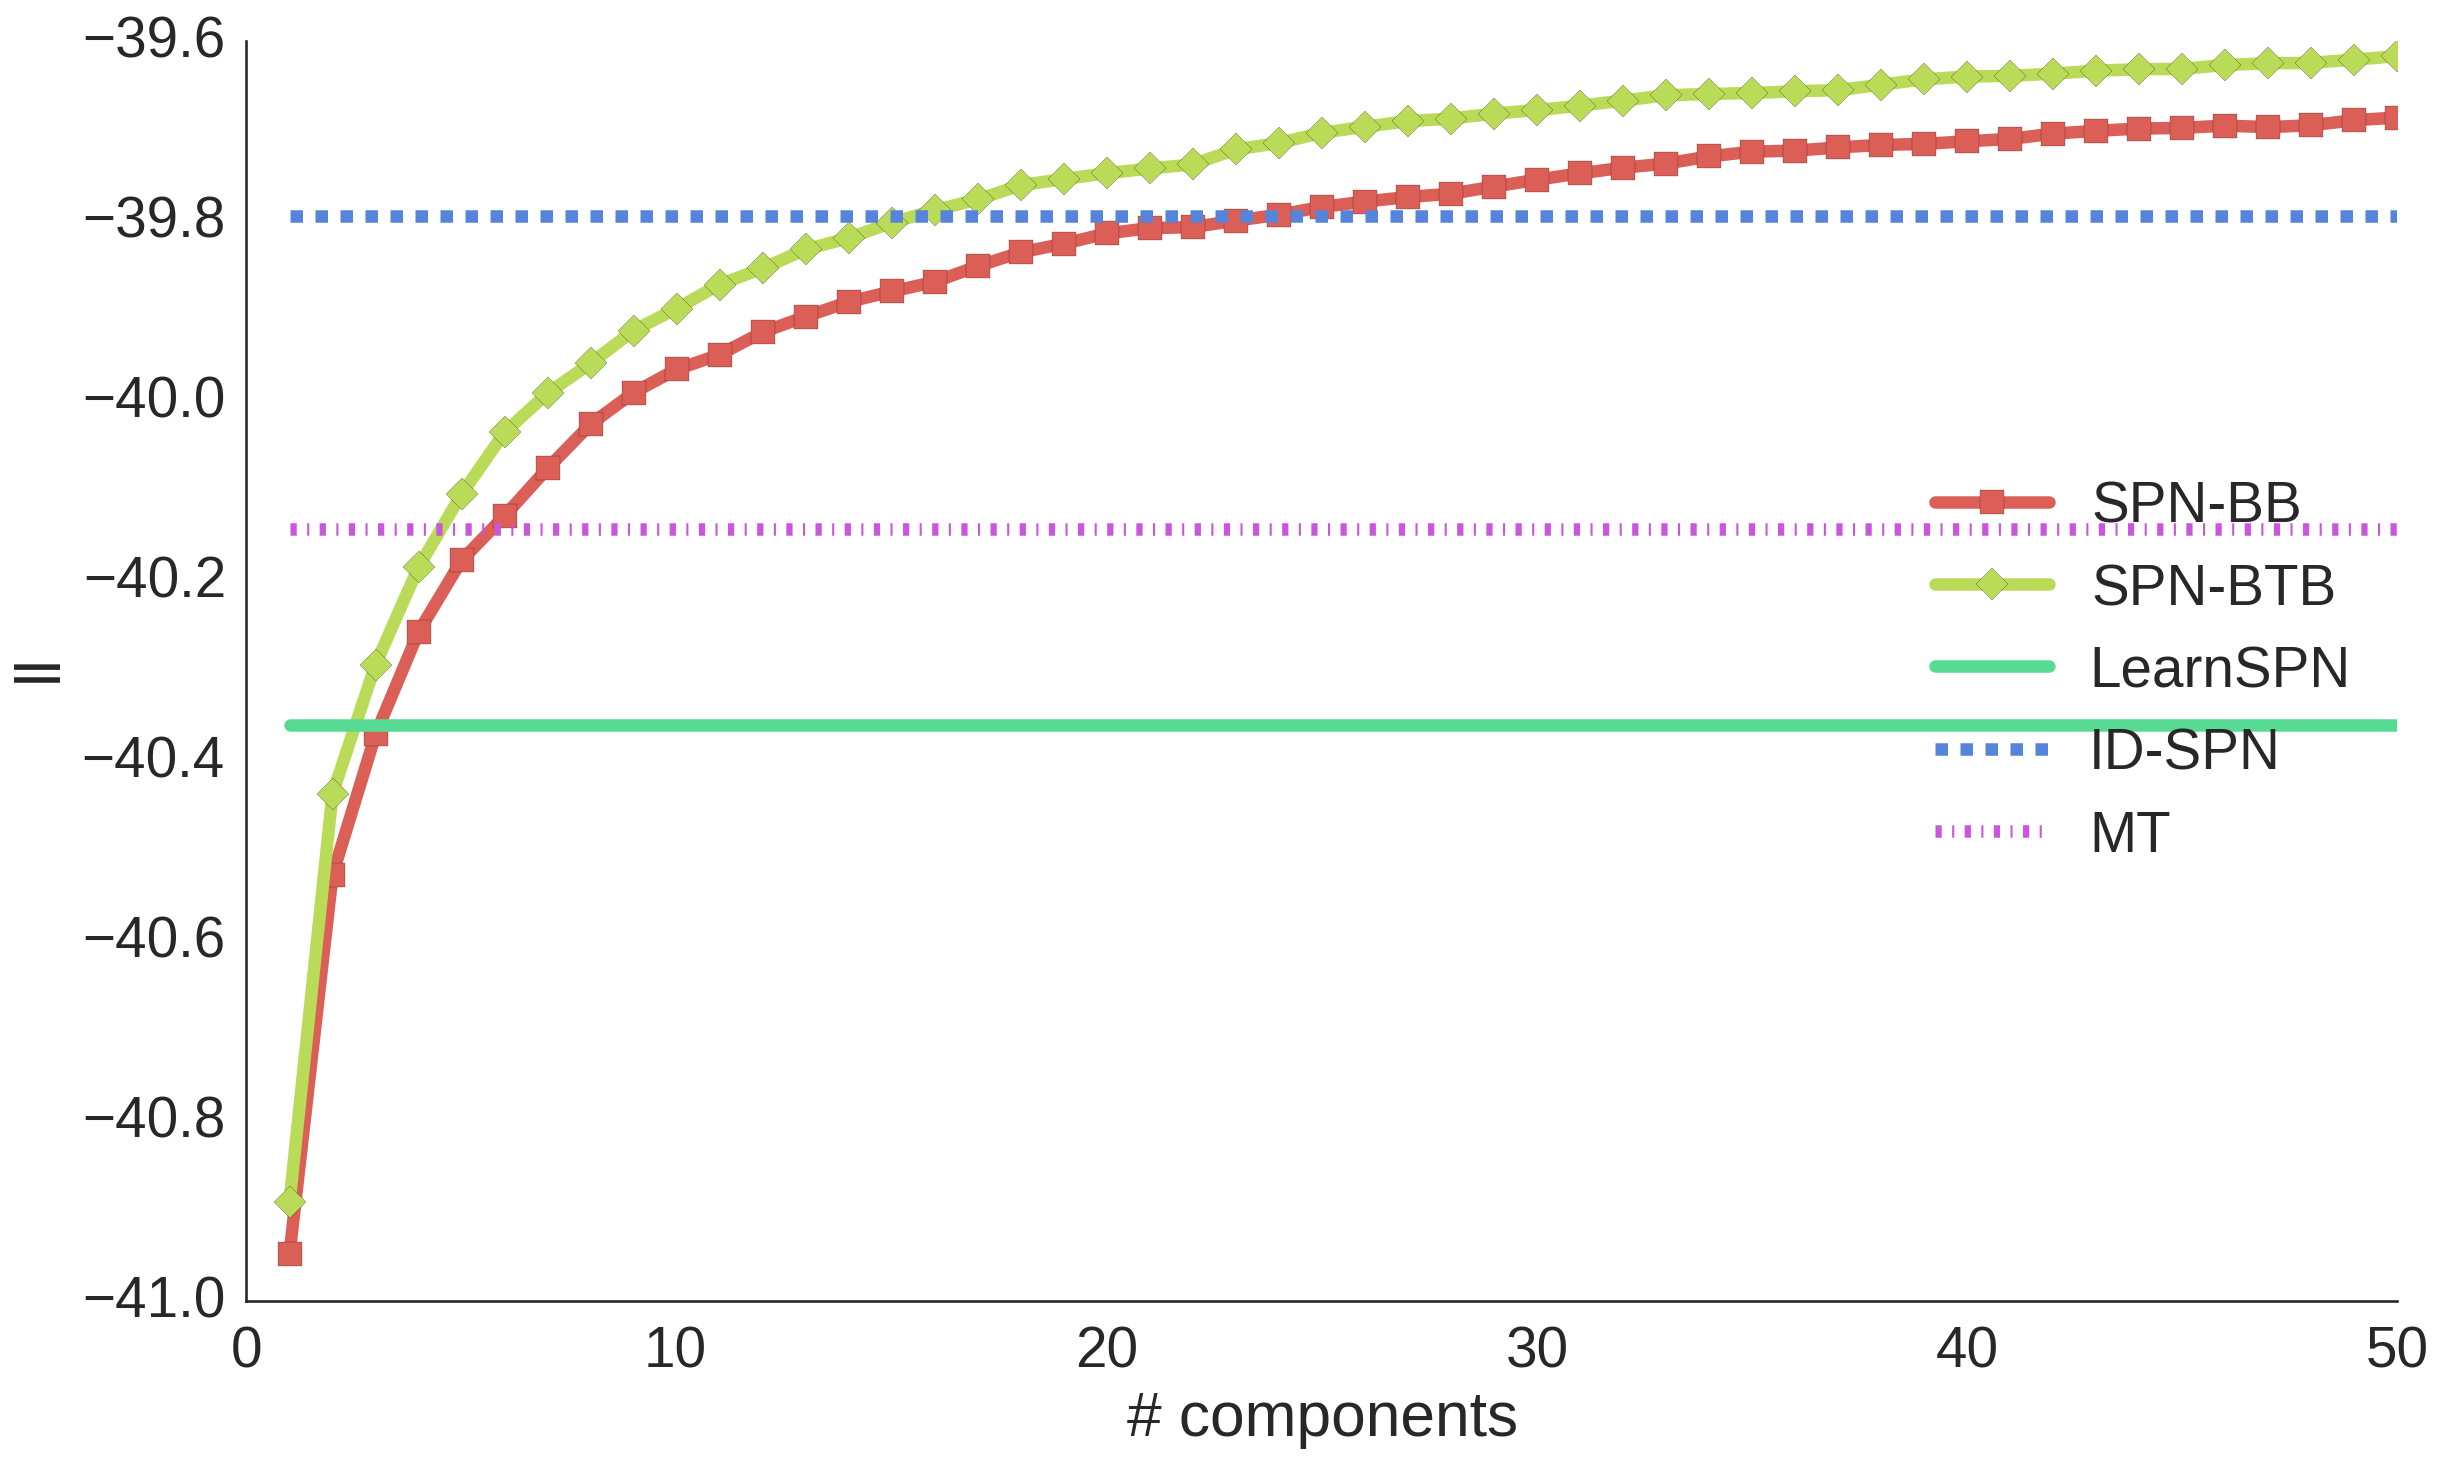
\includegraphics[width=0.4\linewidth]{figures/curves/baudio}&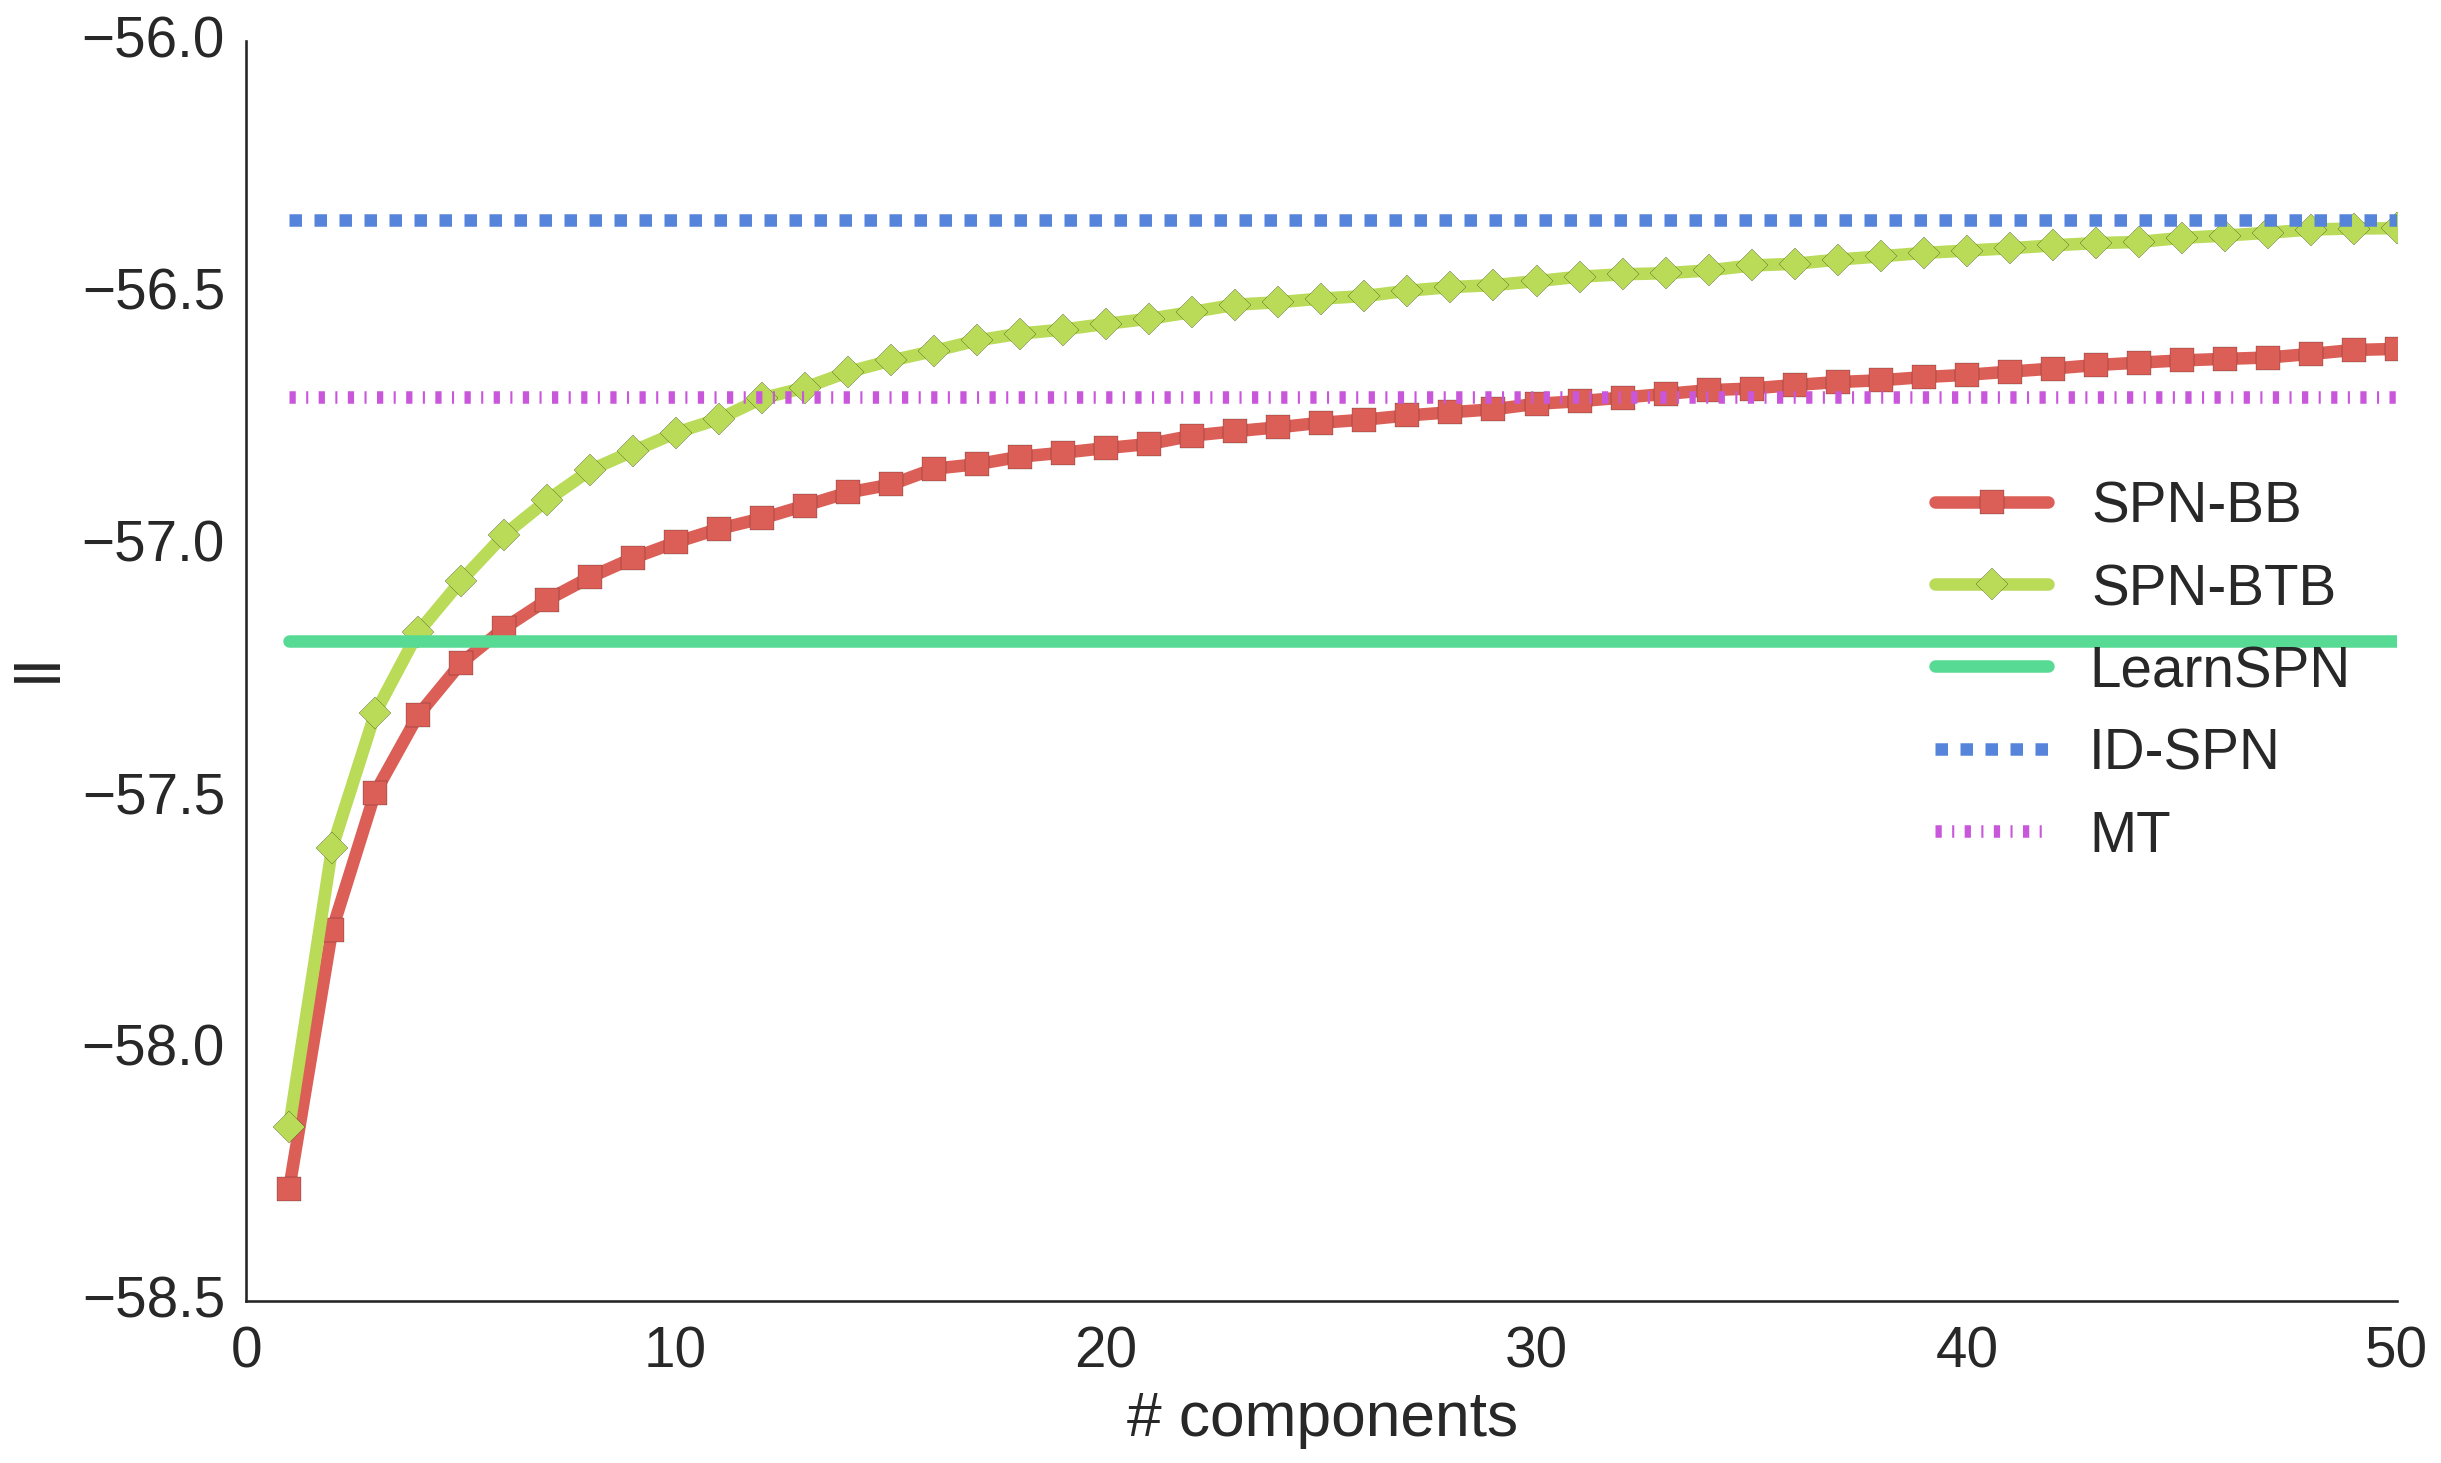
\includegraphics[width=0.4\linewidth]{figures/curves/bnetflix}\\
      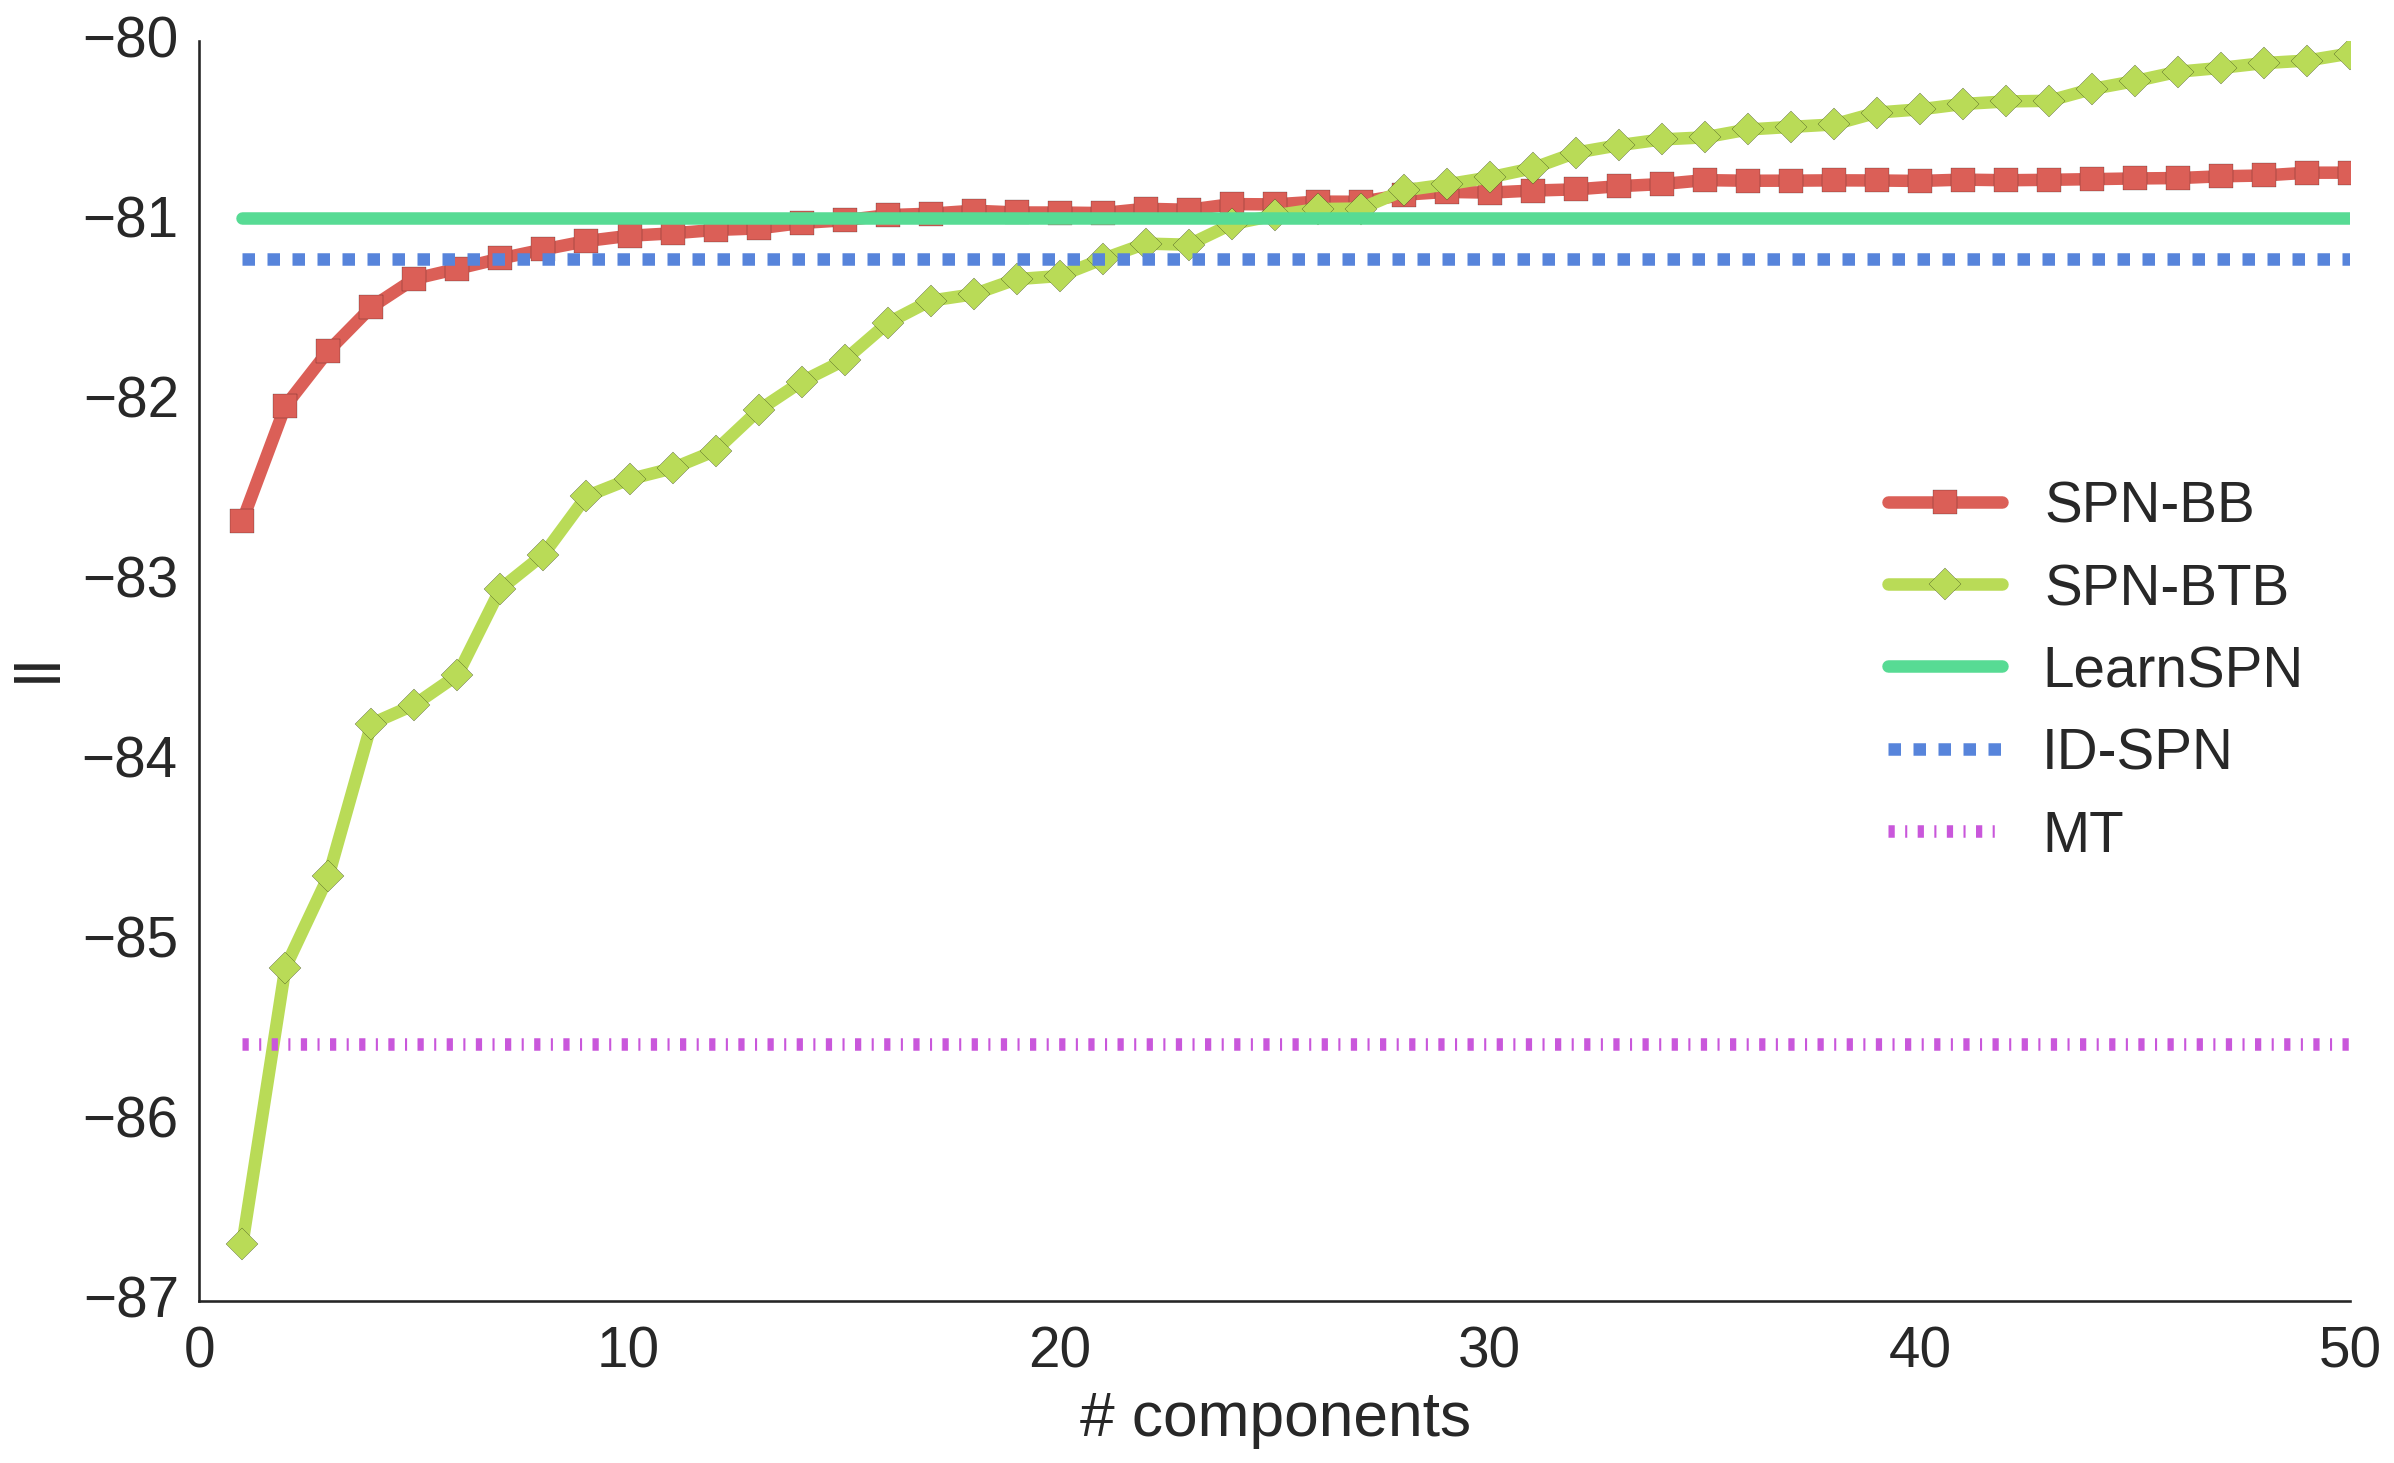
\includegraphics[width=0.4\linewidth]{figures/curves/dna}&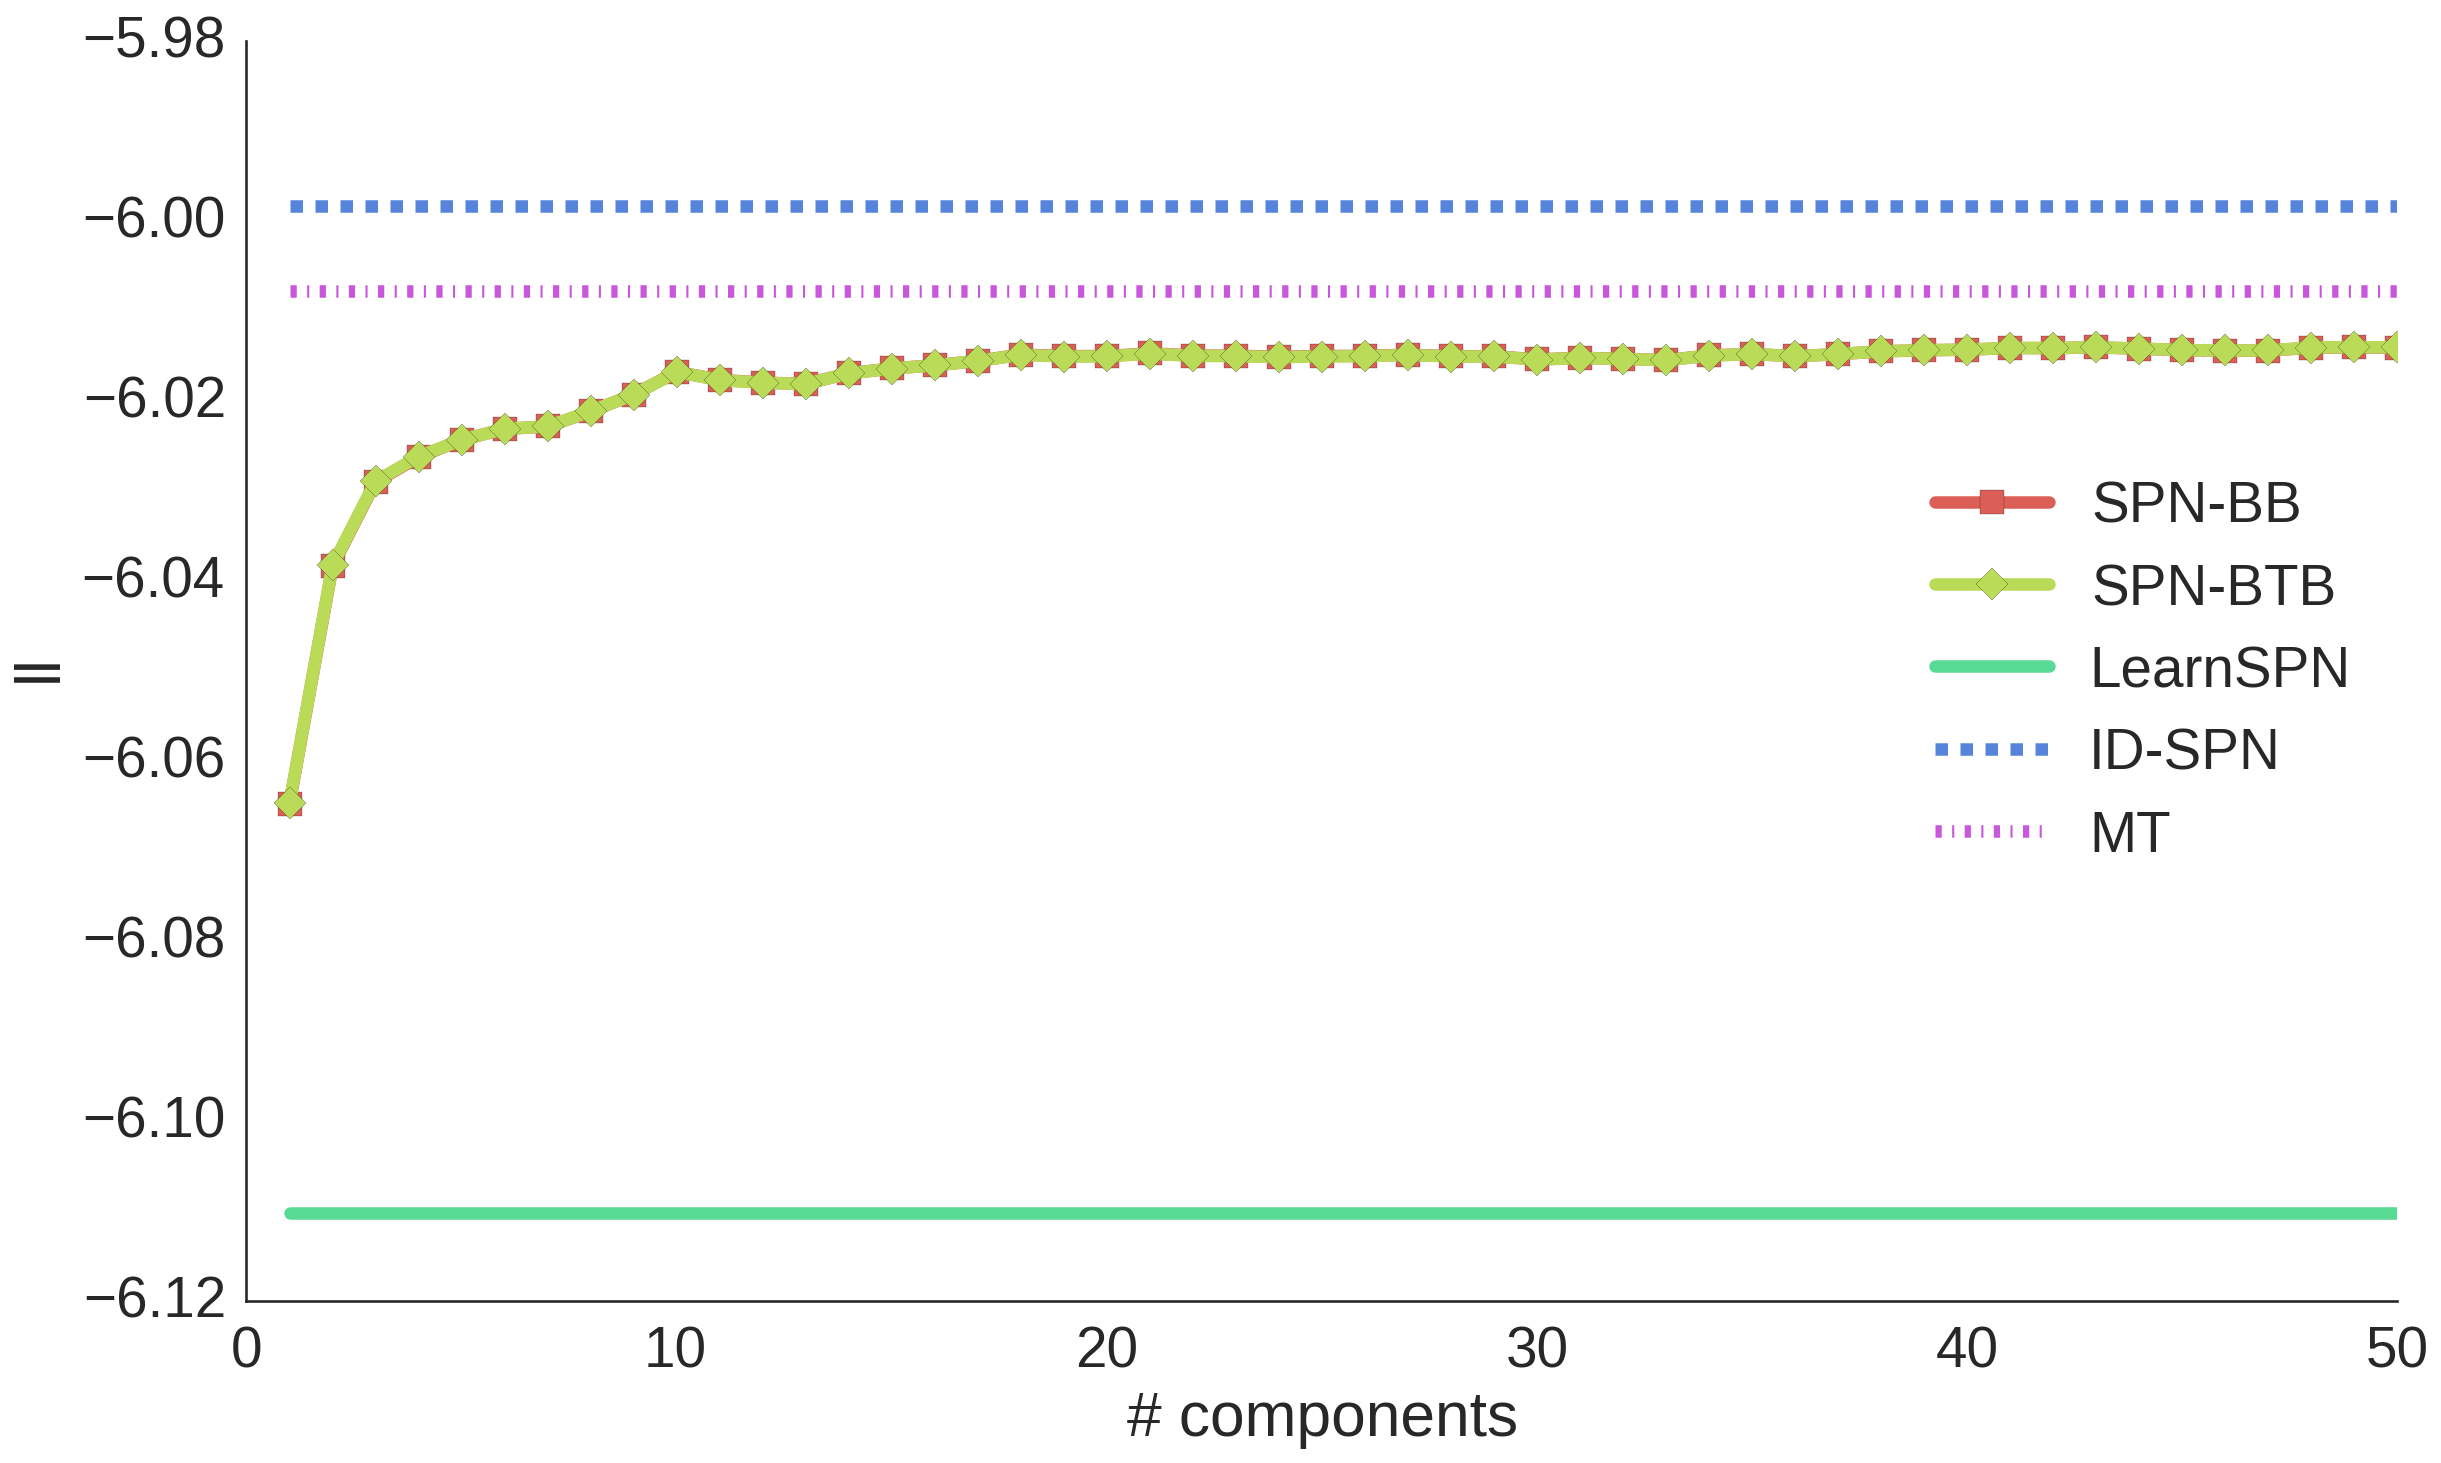
\includegraphics[width=0.4\linewidth]{figures/curves/nltcs}\\
    \end{tabular}
  \end{table}
\end{frame}

\begin{frame}
  \frametitle{Conclusions and Further work}
  \begin{itemize}
  \item Structure quality evaluation matters
  \item Deeper networks by applying a simplicity bias when splitting
  \item Regularized SPNs by introducing Chow-Liu trees as leaves
    \item More robust and accurate SPNs with bootstrapped sum nodes
  \end{itemize}


  
\end{frame}

\begin{frame}
  \frametitle{References}
  \setlength\bibitemsep{8pt}
  \printbibliography
\end{frame}


\end{document}

%%% Local Variables:
%%% mode: latex
%%% TeX-master: t
%%% TeX-engine: xetex
%%% End:
